\documentclass[conference]{IEEEtran}
\IEEEoverridecommandlockouts
% The preceding line is only needed to identify funding in the first footnote. If that is unneeded, please comment it out.

\usepackage{cite}
\usepackage{amsmath,amssymb,amsfonts}
\usepackage{algorithmic}
\usepackage{graphicx}
\usepackage{textcomp}
\usepackage{xcolor}
\usepackage[a4paper, total={184mm,239mm}]{geometry}
\def\BibTeX{{\rm B\kern-.05em{\sc i\kern-.025em b}\kern-.08em
    T\kern-.1667em\lower.7ex\hbox{E}\kern-.125emX}}
\usepackage[utf8x]{inputenc}
\usepackage[colorinlistoftodos]{todonotes}
\usepackage{mathtools}
% \usepackage{tikz,lipsum,lmodern}
\usepackage{tikz}
\usepackage[most]{tcolorbox}
%\usepackage{bm}
\usepackage{enumitem}
\usepackage{csquotes}
\usepackage{makecell}
\setlength{\textfloatsep}{0.5\baselineskip plus 0.2\baselineskip minus 0.5\baselineskip}
\graphicspath{{\pathFigures/}}
\newcommand*{\pathFigures}{figs-final}

\usepackage{amsthm}
\theoremstyle{definition}
\newtheorem{exmp}{Example}[section]

%\usepackage[parfill]{parskip}

\newcommand*\circled[1]{\tikz[baseline=(char.base)]{
    \node[shape=circle,fill,inner sep=0.1pt,font=\footnotesize] (char) {\textcolor{white}{#1}};}}
\newcommand{\boxrj}[1]{\todo[color=green!20,inline,caption=""]{\textbf{Rodolfo}: #1}}
\newcommand{\inlinerj}[1]{{\color{green!40!black!60} #1}}
\newcommand{\inlineisa}[1]{\todo[color=red!20,inline,caption=""]{\sffamily{\textbf{Ingo}: #1}}}
\newcommand{\inlinerc}[1]{\todo[color=yellow!20,inline,caption=""]{\sffamily{\textbf{Rui}: #1}}}

%\author{Fahimeh Bahrami, Ingo Sander, Rui Chen and Rodolfo Jordao\\ KTH Royal Institute of Technology \and Mats Ekman and Ingemar Söderquist \\ {Saab AB, Sweden}}
% \author{Author\\Electronics and Embedded Systems\\School of EECS\\KTH Royal Institute of Technology\\Kistag{\aa}ngen 16\\S-164 40 Kista, Sweden\\\texttt{author@kth.se}}
\definecolor{codegreen}{rgb}{0,0.6,0}
\definecolor{codegray}{rgb}{0.5,0.5,0.5}
\definecolor{codepurple}{rgb}{0.58,0,0.82}
\definecolor{backcolour}{rgb}{0.95,0.95,0.92}

\lstdefinestyle{mystyle}{
  backgroundcolor=\color{backcolour}, commentstyle=\color{codegreen},
  keywordstyle=\color{magenta},
  numberstyle=\tiny\color{codegray},
  stringstyle=\color{codepurple},
%  basicstyle=\fontsize{7}{7}\selectfont\ttfamily
  basicstyle=\fontsize{7}{7}\ttfamily,
  breakatwhitespace=false,         
  breaklines=true,                 
  captionpos=b,                    
  keepspaces=true,                 
  numbers=left,                    
  numbersep=5pt,                  
  showspaces=false,                
  showstringspaces=false,
  showtabs=false,                  
  tabsize=2
}

\lstset{style=mystyle} 
\begin{document}

\title{Systematic Transformational Design for Safety-Critical Embedded Systems\\
%\thanks{Identify applicable funding agency here. If none, delete this.}
}

\author{
  \IEEEauthorblockN{XXXXXXXXXXXXXXXXXXXXXXXXXXXXXXXXXXXXXXXXXXXXXXX}
\IEEEauthorblockA{XXXXXXXXXXXXXXXXXXXXXXXXXXXXXXXXXXXXXXXXXXXXXXXXXXX \\
  \textit{XXXXXXXXXXXXXXXXXXXXXXXXXXXXXXXXXXXXXXXXXx}\\
XXXXXXXXXXXXXXXXXXXXXXXX}
}
% \IEEEauthorblockN{1\textsuperscript{st} Given Name Surname}
% \IEEEauthorblockA{\textit{dept. name of organization (of Aff.)} \\
% \textit{name of organization (of Aff.)}\\
% City, Country \\
% email address or ORCID}
% \and
% \IEEEauthorblockN{6\textsuperscript{th} Given Name Surname}
% \IEEEauthorblockA{\textit{dept. name of organization (of Aff.)} \\
% \textit{name of organization (of Aff.)}\\
% City, Country \\
% email address or ORCID}
% }

\maketitle

\begin{abstract}
Raising the level of abstraction is considered as a key to address the ever-increasing complexity in embedded system design, but it causes additional challenges due to the larger abstraction gap between the initial specification and the final implementation. This paper addresses the current lack of systematic design methods by proposing a  design methodology that extends the existing approaches based on design transformation. Starting with the initial requirements, the proposed methodology advocates semi-formal step-wise transformations to yield a model containing enough synthesis information. At each step of transformation, the system model comprises a set of decomposed and derived requirements, an application model, a platform model, and a set of mapping decisions -- at least one of them is transformed. Each transformation comprises of three steps: 1) possible transformations are identified using pattern recognition, 2) the system model is transformed, and 3) finally, the most promising sequence of transformations is determined using design space exploration. In contrast to other methods, transformations are applied both on the application and platform model to increase the efficiency of the final implementation and to enable the methodology to determine the suitable architecture. The applicability and potential of the methodology are illustrated by a tutorial example.
\end{abstract}

\begin{IEEEkeywords}
embedded systems, design transformation
\end{IEEEkeywords}

\section{Introduction}
\label{sec:introduction} 

%model-based design
%The aim of transform is to 1) add the implementation-dependent details, and 2) reach to an efficient implementation. 
%transform rules for one app or set of apps. 
%One transformation step should define the network between the nodes
%When there are set of apps, we can consider that the platform is a NoC and one node is for the first app and the rest of the nodes are for the rest of apps. 
%model-based process leading from requirements to implementations \cite{sifakis2014rigorous}.
% while verifying at every step that the design properties  hold \cite{ungureanu2019formal}.
%The underlying MoC in this paper is SDF. Apps which are considered here are Data Flow applications.
%top down transformation methodology for a predictable system design.
%"good enough" solution or "optimal" solution

% Safety-critical embedded systems have undergone a revolution over recent decades;
The design process of safety-critical embedded systems has become very challenging due to increasing functionality and additional demands on safety and performance.
Raising the level of abstraction is regarded as an important technique to manage the complexity of designing today's systems, as it is easier  to  capture  the functionality  of  the  system  at the  higher abstraction  levels. Although this approach has many potential  benefits,  including  decreasing  verification time and costs and  potentially increasing  the degree  of  automation,  it  widens the  gap  between specification and implementation. Naturally, high-level  specification  models  lack  implementation  details, which have to be added during the design process.
% Indeed,  since \emph{implementation-dependent requirements} increase the complexity of the high level specification model, they must be added step wisely during the design process.
A  promising technique to systematically add information, requirements and details to the initial model and fill the gap is to use a transformation-based  approach. This is also supported by the arguments of \cite{kahng2009orion}, stating that \textquote{high-level optimizations have been shown to have much more significant impact on power than low-level optimizations.}
%high level design decisions, have been proved to have much more effect on the  ultimate design rather than the lower ones
%\inlineisa{Check quote!}


%In this work, an extension of the transformational system design methodology introduced in \cite{sander2004system} is developed for the entire design process of predictable systems, from a high abstraction level down to the lower levels.
%In the proposed methodology, the high level design decisions, that have been proved \textquote{to have much more effect on the  ultimate design rather than the lower ones} \cite{kahng2009orion}, are made earlier to avoid iterations of common system design methods like V-model \cite{forsberg1991relationship} and Y-chart \cite{grout2011digital}. 

The proposed methodology in this paper extends the rule-based transformation approach presented in \cite{sander2004system}. Potential transformations can be identified using \emph{patterns}, which together with the \emph{transformed patterns} are part of the transformation rules.
% The \emph{transformed patterns} are also defined in the transformation rules.
A \emph{pattern recognition} method is developed and adopted to detect possible transformations in each step of the design process. The specification model is transformed based on the transformed pattern defined in the applied transformations. Finally, having all options for transformation, the sequence of transformations that makes the best trade-off between different performance metrics, is selected from the candidate sequences of transformations that preserve requirements. Early-stage design space exploration (DSE) in conjunction with traditional DSE techniques are leveraged for this aim.
In the proposed transformational design flow, the whole system model including an \emph{application model}, a \emph{platform model}, a \emph{mapping model}, and  \emph{requirements} is transformed in each step of the design process. By this, a larger part of the design space is traversed, and the possibility to obtain an efficient implementation is vastly improved compared to earlier approaches that only transform the application model \cite{sander2004system} or the platform model \cite{nuzzo2015platform}. To fulfill this aim, the following novel concepts and techniques are introduced:
%the conceptual requirements, i.e., system requirements, and \emph{refined requirements}, i.e., requirements estimated and extracted from the high-level functional specification of the system by the expert designers and the estimation of available performance of the foreseen computation resources and network topology.

\begin{itemize}[leftmargin=*]
	\setlength{\parskip}{1pt} 
	\setlength{\itemsep}{0pt plus 0pt}
 \item \textbf{System model transformation:} To obtain an efficient implementation, a good match between application and platform is key. Thus, transformations can be applied on all parts of the systems model, consisting of \emph{requirements}, \emph{application model}, \emph{platform model}, and \emph{mapping model}.
 \item \textbf{Pattern recognition:} Apart from the highly addressed research problem of how to verify the correctness of a transformation
   % , i.e., if the transformed model preserves the properties
   \cite{broy2012specification, nuzzo2015platform}, it is vital to be aware of all possible transformations in each transformation step. To achieve this aim, a pattern recognition technique is introduced and leveraged for a semi-formal rule-based transformational design approach.
    \item \textbf{Transforming requirements:} In each transformation step, the requirements must match the transformed system model. This requires both decomposing the requirements according to the new subsystems and adding implementation-dependent requirements resulting from design decisions.
\end{itemize}

%\vspace{-0.1in}
%\begin{itemize}
%    \item \textbf{Transformational  ment  methodology:} We propose a methodology for step-wise transformational system design.  The starting point of the transformational flow is a well-defined formal specification model undergoing several refinement steps and ending with a synthesizable implementation model. \emph{Refined requirements} and \emph{parallel transformation} of the application specification model, the platform model, and the mapping, as well as the requirements/constraints are very important concepts introduced and used in the proposed methodology.
%    \item \textbf{Transformation strategy:} We define which transformations, in which order, should be applied to provide an efficient implementation preserving all the requirements. To identify possible transformations, a \emph{pattern matching} technique is introduced.
%    \item \textbf{Platform refinement:} This section will be completed in the final version of the document (deliverable D3.3).
%    \item \textbf{Categorization of transformation rules:} This section will be completed in the final version of the document (deliverable D3.3).
%    \item %should be corrected
%    \textbf{Testing the proposed methodology:} The usage and potential of the presented transformational system design  is exemplified by ForSyDe (Formal System Design) modeling framework and tools \cite{sander2003system}, as well as the interface modeling framework proposed by \cite{hendriks2020interface}. The key insight of using examples is to show the effectiveness of the refinements enabled thanks to our transformational design flow in a broad range of applications.
%    \item \textbf{Reliability:}
%\end{itemize}

%Table \ref{terminology} defines the terminology used in this paper. 


%model-based development
% a systematic formal methodology
The scope of the paper is to introduce a semi-formal transformation-based technique for different application domains wrapped in a systematic design methodology to keep a uniform and functional view of the design, where also non-functional requirements are captured.
% Moreover, this paper investigates the methodological issues of transformation-based development.
We aim for a semi-formal and semi-automated design methodology and to lay its foundations in this work; detailed suggestions and tool support  of the transformations will be addressed in future work. 

The paper uses a tutorial, but representative example, to illustrate the central concepts and techniques introduced and developed in this work. The main objectives are to 1) show the effectiveness of our integrated methodology, 2) clarify its viewpoint on system design as a series of transformations, 3) demonstrate the level of design automation can be increased. 
%It should be noted that in the current work, the terms ``transformation'' and ``refinement" are used interchangeably. 

%The rest of the paper is organized as follows. Section~\ref{sec:system model} describes the system model.
%followed by the problem statement in Section~\ref{sec:problem-statement}. 
%Our proposed transformational system design methodology is detailed and exemplified in Section \ref{sec:transform-methodology}. 
%Transformation rules are classified and explained in Section \ref{sec:classification}. 
%The usage of the introduced methodology is illustrated by tutorial examples in Section \ref{sec:test}. 
%Section~\ref{sec:related-work} investigates the related work in detail and,
%Finally, a conclusion is given in Section~\ref{sec:conclusion}.  


%%% Local Variables:
%%% mode: latex
%%% TeX-master: "../paper"
%%% End:

\section{System Model}
\label{sec:system model}
\begin{figure}[t]
	\centering
   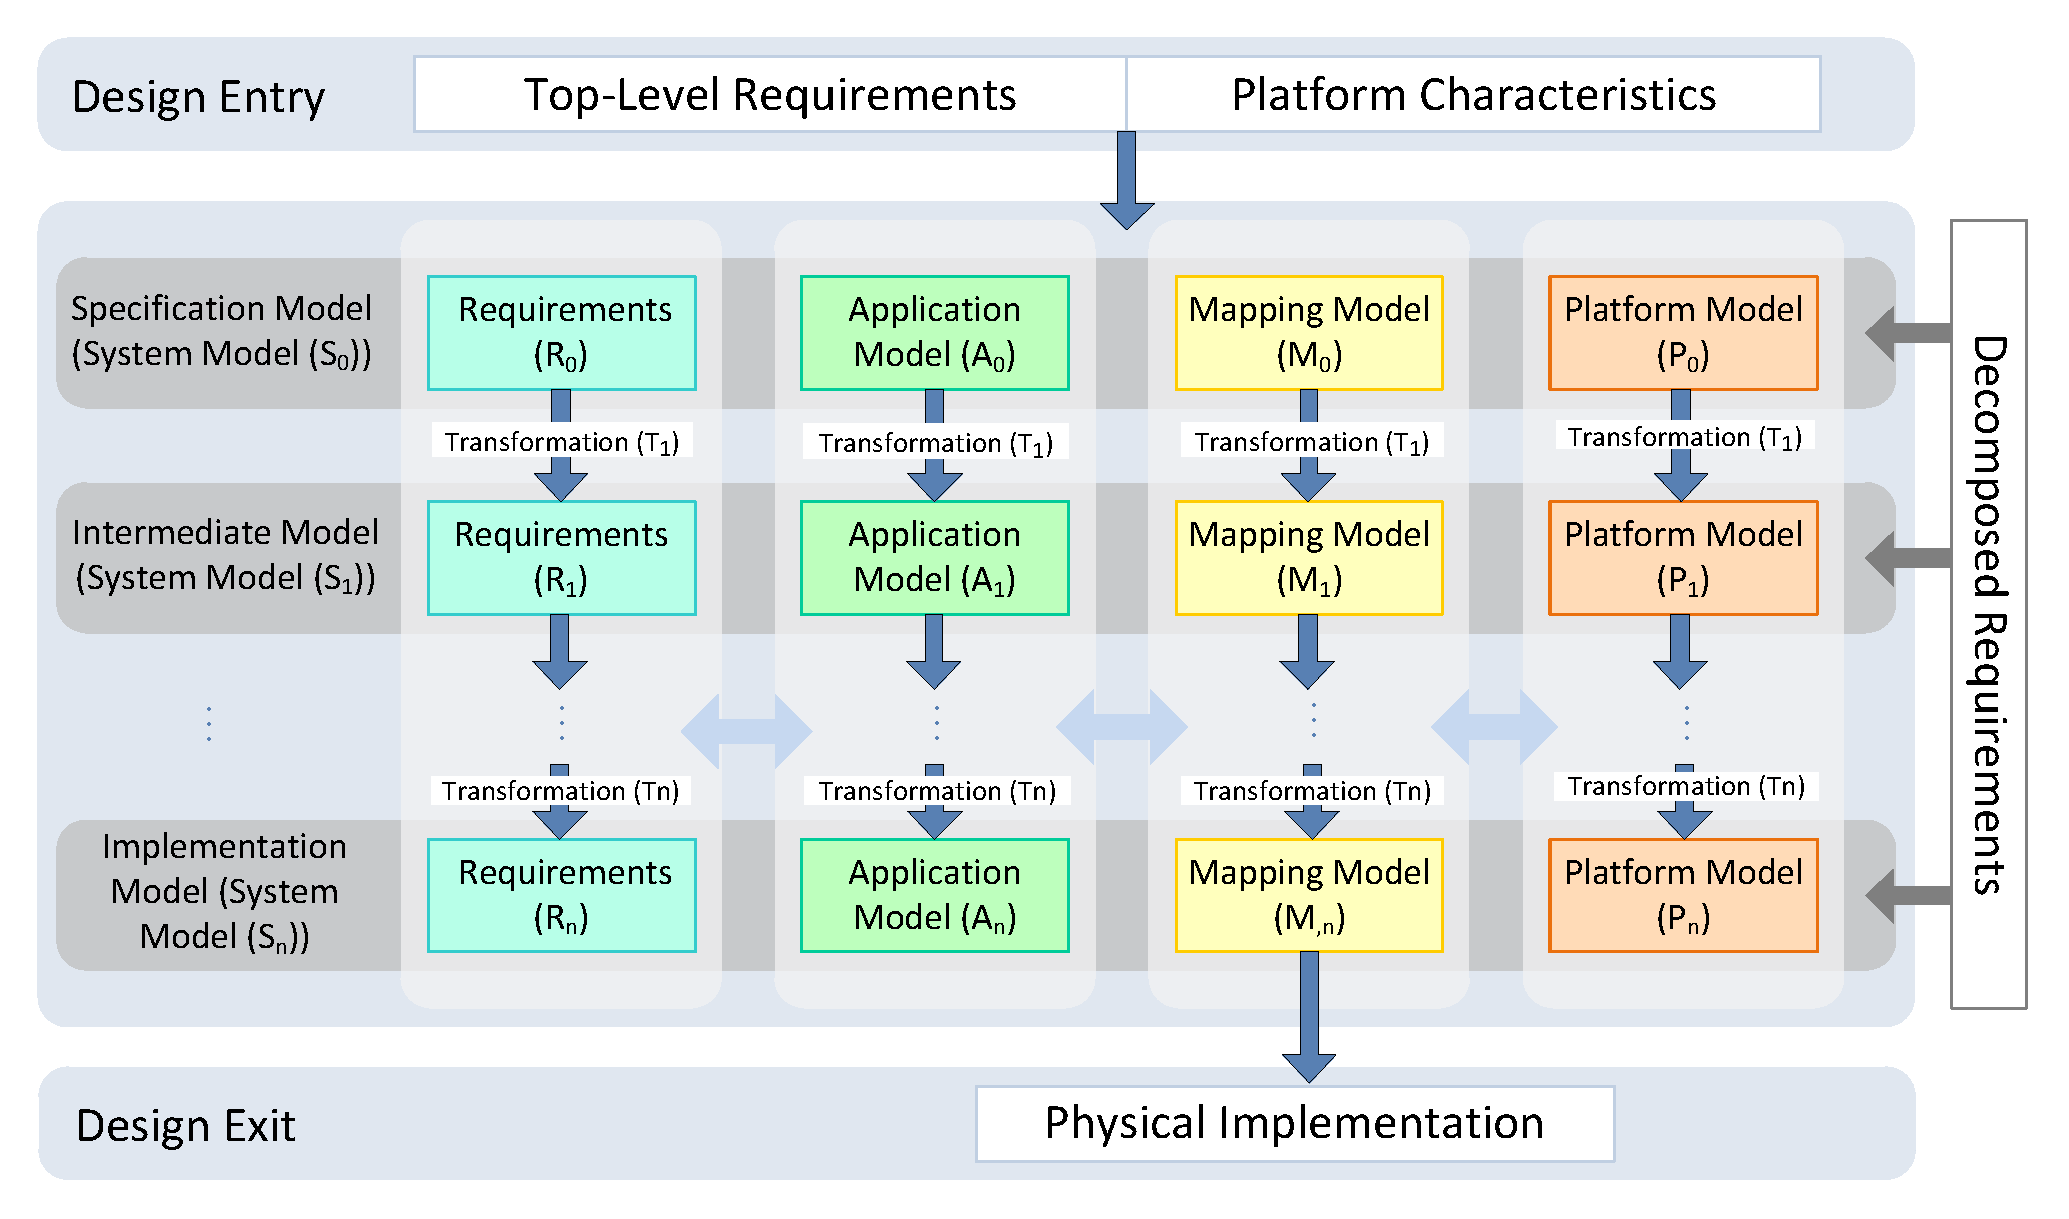
\includegraphics[width=\columnwidth]{figs-src/system-model.pdf}
	\caption{System model transformation.}
	\label{sequence}
\end{figure}

The system design process consists of a sequence of transformations, i.e., $\Gamma = \left \{T_0, T_1, ... , T_n \right\}$, with different granularity levels (Figure \ref{sequence}). At the higher abstraction levels, transformations are usually coarse grain and have been proved to have major effects on  the physical implementation \cite{kahng2009orion}. The transformation process continues until the model contains sufficient information for the synthesis to a target platform.   

In this transformation-based system design approach, a \textit{system model} $S$ is considered to consist of \textit{requirements} $R$, an \textit{application model} $A$, a \textit{mapping model} $M$, and a \textit{platform model} $P$, i.e., $S =(R,A,M,P)$. The system model is shown in Figure~\ref{sequence} and explained in the following sections. We refer to the system model in different transformation steps as \textit{RAMP}, implying slopes that connect the specification model on the highest abstraction level to the final implementation.  The vertical arrows in Figure \ref{sequence} demonstrate potential transformations, i.e., at least one of the parts of the system model is transformed at each step. The methodology allows transformations in all parts to mix and match them after each transformation.
%Table \ref{notation} denotes  all  important  notations. 
Note, that a clear separation between the application model and the platform model is emphasized in our methodology. This feature allows the designer to continuously refine both application and platform models to identify an efficient implementation.

\subsection{Application Model}
\label{sec:application model}
In our methodology, an application is considered as a function over signals.
% Because some behavior of a system that are generally considered as side effects, e.g. writing data to a register, can be formulated by a stream of its history.
This abstraction is powerful to express systems in the domain of pure functions, which provides a sound base for formal analysis. Further, we introduce models of computation (MoCs) \cite{LeeSan1998} and parallel skeletons \cite{Cole1989a,Ski1994} to model the application. This enables to explicitly specify the temporal properties and potential parallelism of an application and makes it possible to define transformations which make effects on different aspects separately. Both MoCs and skeletons can be defined as high order functions (HOFs). Hence, a consistent syntax and semantics can be defined for transformations on MoCs, skeletons or the whole application models.
%The proposed methodology supports the application models based on a  sound formal base in form of the theory of models of computation (MoC) \cite{JanSan2005a}. More specifically, the application model should be based on:
\begin{itemize}[leftmargin=*]
	\setlength{\parskip}{1pt} 
	\setlength{\itemsep}{0pt plus 0pt}
    \item \textit{Process constructors:} Following \cite{sander2004system}, the application models are process networks in which concurrent processes communicate with each other via signals. Also, in such application models, a clean separation between computation and communication is achieved by means of the concept of process constructors. A process constructor is a HOF, which takes pure functions and values as arguments, and creates a process. The process constructor describes the communication interface of the process, while the arguments to the process constructor describe the computation of the process. This clean separation is important for our transformation-based design process, since it enables to define transformation rules for processes, which have the same process constructors, but have different arguments.
    \item \textit{Skeletons:} Data-parallel skeletons enable transformations that exploit potential parallelism \cite{Cole1989a,Ski1994}. Skeletons enable to express parallel patterns and have been used to model abstract building blocks that have a predefined implementation on a parallel machine. 
\end{itemize}

Our methodology uses skeletons in tandem with process constructors to enable the transformation of application models into efficient parallel structures for which an efficient implementation in hardware and software exists.

\subsection{Platform Model}
\label{sec:platform model}

For the platform model, we follow the typical platform-based design (PBD) frameworks and highlight the features that a framework should have to support transformational view that the methodology needs \cite{attarzadeh2014framework}, \cite{nuzzo2015platform}, \cite{hendriks2020interface}. 

The  methodology  targets \textit{predictable platforms}  with  guaranteed  performance  metrics. The platform model is  built out of a library of initial components. The components are building blocks, and therefore the platform model is a block diagram consisting of interconnected
building blocks. The library should be rich enough to model different components on the set of alternative platforms. In addition, functionality of the components, i.e., what the components do, in the component library need to be in line with the constructs to build the application model. In other words, there should be hardware and software interpretations of process constructors and processes, i.e., building blocks of the application model, with determined performance metrics in the component library. Components are characterized by parameters and control functions, and therefore can model different configurations, as well as their performance metrics. Composition rules of the components, for creating a valid platform, should be also fed into the design process. 
%The framework should provide formal notations for the mentioned characteristics to enable \textit{compositional design} and \textit{compositional verification}. 
The part of the methodology related to refining the platform model pursue the goal of instantiating the components and composing them to obtain an efficient architecture that satisfies both functional and non-functional requirements.


%Furthermore, the platform modeling framework should share the same view of characterizing components with interface models \cite{hendriks2020interface} to support \textit{compositional refinement}, i.e., to refine an interface to blocks communicating with each other that implement the given interface \cite{hendriks2020interface}. Interface models are more restricted in terms of the environment, i.e., the inputs to the component (very similar to the input assumptions in assume/guarantee contracts \cite{nuzzo2015platform}, \cite{broy2012specification}). This feature of interface models lay the foundations for compositional refinement as for each component, it describes how to use a component and how it can be composed with other components. 

\subsection{Mapping Model}
\label{sec:mapping model}

For the mapping model, we use the simple but useful design space modeling technique carried out in \cite{blickle1998system}. The application model, i.e., a process network, and the platform model, i.e., a block diagram, are represented as graphs.
As they are, by construction, bipartite \cite{diestel2010graph}, the mapping model consists of edges between them, embodying any possible mapping. This
definition implies that the application and platform models must have
a \emph{corresponding} graph represention, but need not to be graph models
themselves.

\subsection{Requirements}
\label{sec:requirements}

We distinguish between traceable and untraceable requirements. System requirements are classified to \textit{decomposed requirements} and \textit{derived requirements} \cite{johnson1998178b}, \cite{landi2011arp4754a}. Decomposed requirements are top-level requirements decomposed to more detailed ones to be assigned to different subsystems. These requirements should be traceable forward and backward and should be verified after each transformation step. The requirements tree in Figure \ref{specification} illustrates decomposed requirements. However, in a design process, there are some design decisions that previously were made by designers. These design decisions are implementation-dependent and can not be captured at the higher abstraction levels. Instead, they are captured as derived requirements at the lower levels by rule-based algorithms describing acceptable decisions. Derived requirements can not be traced, however, they are powerful levers for transformations. In other words, the designer's knowledge is injected to the design flow as derived requirements and used as guidelines to achieve an efficient implementation during the transformation phase. Examples of derived requirements are requirements on robust partitioning, validity check of incoming data, redundancy, as well as requirements on maximum power consumption, computational load, and  network capacity utilization. 

%Examples of derived requirements are the execution frequency and estimated memory space needed for each task, the size of the buffers, data types, energy rules, and safety related requirements.

%\subsection{Refinements}
%\label{sec:refinement}

%The system model $S$ in transformation step $m$ is represented by the 4-tuple $S_m: (R_{i}, A_{j}, M_{k}, P_{l})$, in which $0 \leq i,j,k,l \leq m$. The indices $i,j,k,l$ shows the last transformation step in which the corresponding element is changed. In each transformation step at least one of the elements of the 4-tuple change. i.e., $(i=m) \vee (j=m) \vee (k=m) \vee (l=m) = 1$. For example, the transformation 

%$S_{m-1} \xRightarrow{T_m} S_{m}$, in which

%$S_{m-1}: (R_{m-1}, A_{m-1}, M_{m-1}, P_{m-1})$

%$S_{m}: (R_{m-1}, A_{m}, M_{m}, P_{m-1})$\\
%shows that during transformation step $m$ only the application model $A$ and the mapping model $M$ are refined. As a practical example, if the target platform is given from the beginning of the design process, $\forall m: P_{m} =~P_{0}$.

 

%%% Local Variables:
%%% mode: latex
%%% TeX-master: "../paper"
%%% End:

%
\section{Problem Statement}
\label{sec:problem-statement}

%Embedded systems need more automated and efficient system development methodologies to enable capability growth, and thereby increased complexity with retained acceptable development cost and time. Current design flows for conceptual system development, down to hardware and software development, do not have a clear path from the functional specification down to the final implementation and cannot provide guarantees on performance metrics early at the conceptual phase. 



%From aeronautics industry point of view, such systems need more automated and efficient system development methodologies to enable capability growth and thereby increased complexity with retained acceptable development cost and time. The avionics system based on electronics and software is a prerequisite for an aircraft’s general functions. Current design flows for conceptual system development, down to hardware (electronics) and software (code) development, do not have a clear path from the functional specification down to the final implementation and cannot provide real-time guarantees early at the conceptual phase. hallenges with the never-ending growth in number of functions as well as their complexity in an aircraft and the architecture change from several dedicated resources for each function to shared heterogeneous resources connected in a network with computation nodes and I/O enforces the necessity to increase the use of formal methodologies applied at early conceptual design. Thereby move focus away from the today often seen on low-level simulation, analysis, and verification. It is also essential to address the recognized challenge that early system design decisions, combined with lack of experience and continued follow-up on foreseen resource needs, often lead to very late and costly changes in the overall architecture. Suggested industrial design flow with specifications written in a formal language allow automated verification process to start early in the design process and at high abstraction levels without the need to code several new verification models. This enables an integrated design flow from specification to a completed system that can be completely validated at each step between abstraction levels, e.g., refined estimates on resource needs.
 
From a more general and, in the mean time, detailed view of system design process,  verification  cost  is  a  major  part  of  embedded system design costs, especially for systems with compulsory certification requirements, as a consequence of the increasing  tendency  for  taking  advantage  of  high-performance  and  cost-effectiveness  of  complex  heterogeneous  systems-on-chips  (SoC).  The  common technique  for  verification  is  simulation  which  is  a time-consuming  and  costly  technique, especially for real-world tests that even can not be done till late stages.  Instead,  formal  verification  is  a  promising  method  to  alleviate the burden  of  verification.  Formal  system  design  approach is  recognized  as  the  first  step towards this  aim.    It  starts  with  a formal  specification model at  a  high  level  of  abstraction  which  is free from implementation details and, therefore, is easy to verify.  Also, the simplification causes designers to focus their effort on the functionality of the  system,  which  in  turns  increases  the  accuracy  of the specification modeling phase.  Moreover, the simpler model, the less complex verification technique is needed.  On the  other hand,  the higher  abstraction level, the larger gap is made between the specification and  the  implementation  model.  However,  the  implementation details are of great importance to reduce the design space and achieve an efficient implementation.  As a result, they should be added step wisely during a transformational  refinement  process. 
%Each step of this process is an effort to add one of the required properties, e.g., constraints and performance indexes,  given  in  the requirement  specification,  to  a system  model  at  one  abstraction  level  and  produce another model at the same or lower abstraction level. Design space reduction is also one of the achievements of this process. 
Preserving properties during the transformations is another challenge that the underlying transformation methodology should deal with. In this study, we introduce a transformation-based design methodology  to address all the mentioned challenges. The proposed methodology is an efficient development approach and increases the level of automation. It has a clear path from the functional specification down to the final implementation and can provide guarantees on performance metrics early at the conceptual phase. Another recognized design challenge in industry that the introduced methodology meet is that early system design decisions, combined with lack of experience and continued follow-up on foreseen resource needs, often lead to very late and costly changes in the overall architecture. Thanks to transformational desgin view exploited in our methodology, design decisions are made early in the design process, and verification process starts at higher abstraction levels without the need to code several new verification models. This enables an integrated design flow from specification to a physical implementation that can be completely validated at each step between abstraction levels.



%Figure illustrate the step wise process and its effect on the design space.


%\begin{figure}[htbp]
%  \centering
%  \scalebox{0.8}{\input{\pathFigures/abstraction-gap-refinement.pdf_t}}
%  \caption{The synthesis process is a stepwise refinement from a high-level specification model into a final implementation}
%  \label{fig:abstraction-gap-refinement}
%\end{figure}


%%% Local Variables:
%%% mode: latex
%%% TeX-master: "../paper"
%%% End:


\section{Transformational Design}
\label{sec:transform-methodology}
\begin{figure}[t]
	\centering
	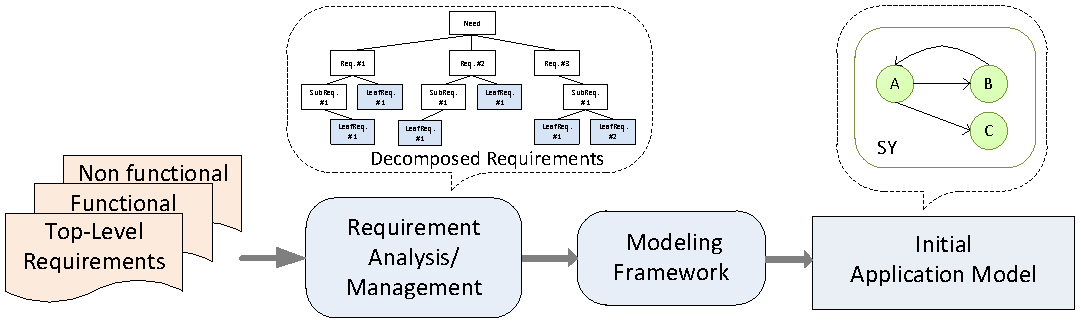
\includegraphics[width=\linewidth]{figs-src/specification.pdf}
	\caption{Specification phase of the proposed methodology.}
	\label{specification}
\end{figure}

The operational flow of the proposed transformation-based methodology is shown in Figure \ref{specification} and \ref{transformation} (in the following, words in \textit{italics} refer to the corresponding part in these figures). It comprises two main phases: 1) specification phase, and 2)  transformation phase, which belong to at least two  abstraction levels: the functional abstraction level and the functions decomposed to components abstraction level. The phases are elaborated and demonstrated by a running tutorial, but representative, example of a typical image processing application throughout this section. The goal is to show the use of our methodology and to explain the introduced concepts and techniques. 

%The operational flow of the proposed transformation-based methodology is shown in Figure \ref{specification} and \ref{transformation} (in the following, words written in \textit{italics} refers to the corresponding part in these figures). It comprises two main phases: 1) Specification phase, 2)  transformation phase, which belong to at least two  abstraction levels including the functional abstraction level and the functions decomposed to components abstraction level, respectively. The phases are elaborated in the following and are demonstrated by a running example of a typical image processing application throughout this section. The goal is to show the use of our methodology by this tutorial, but representative example and to explain the introduced concepts and techniques. 

\subsection{Specification Phase}
Figure \ref{specification} shows the specification phase of our transformational design flow. The starting point is requirement specification. The requirements that are usually in text format (\textit{Top-level Requirements}), are specified by means of an executable model. This step of design starts with breaking functional and non-functional requirements into several sub-requirements, so-called \textit{Decomposed Requirements}, and continues to  decompose them to smaller ones (\textit{Requirement Analysis/Management Tool})~\cite{grady2010system}. The result of this step is a requirements tree. It should be noted that the requirements will be further decomposed to be assigned to sub-systems, and the requirements tree will be extended and used for tracing decisions and their implications on other requirements during the transformation phase. At the next step of requirement specification, the leaf nodes of the requirement tree are associated with a set of functions by means of the chosen formal functional modeling framework (\textit{Modeling Tool}). These functions are arguments to the higher-order functions, i.e., process constructors and skeletons, and will not be touched and further refined during the transformation process. Therefore, the smaller the requirements in the leaf nodes of the requirements tree, the more opportunities for transformation in the transformation phase. The output of specification phase is an \textit{Initial Application Model} which at least specify all the functional requirements and is ready to be further refined in transformation phase of a design to include non-functional and implementation-dependent requirements, so-called \textit{Derived Requirements}, as well. Example \ref{ex:appModel} is an example of the specification model of the image processing application. 

\begin{figure}[t]
%    \captionsetup{position=b}
	\centering
	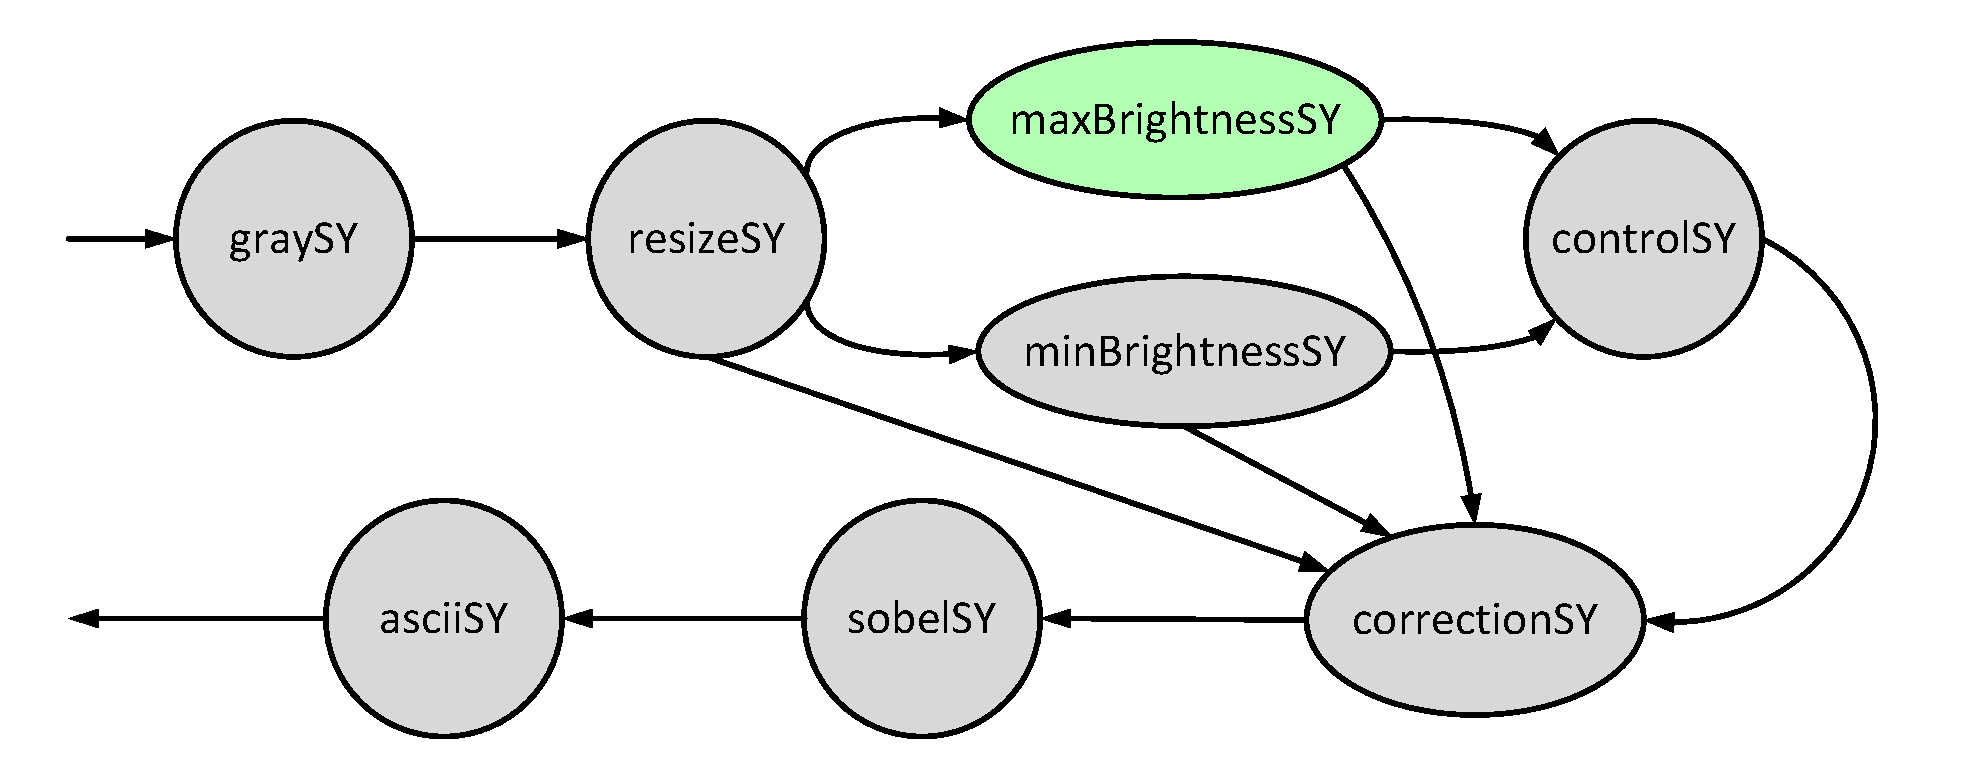
\includegraphics[width=2.3in]{figs-src/appModel.pdf}
	\caption{Image processing application model.}
	\label{appModel}
\end{figure}

\begin{exmp}\label{ex:appModel}
Figure \ref{appModel} illustrates the application model of an image processing application that converts an RGB-image to an ASCII art image, using brightness correction and edge detection (Sobel).
The application model is specified using ForSyDe \cite{sander2004system}, which has the features discussed in Section \ref{sec:application model}. It is based on the synchronous MoC and skeletons. 
In the synchronous MoC, a signal $s$ is modeled as a sequence of events, where each event $e_i$ has a tag and a value: $s = \{e_0, e_1, \dots\}$. The tag is implicitly given by the position of the event in the signal. A vector $v$ of $m$ elements is denoted by $v = [v_0, v_1, \dots, v_{m-1}]$. The process constructor $\mathit{mapSY}$ applies a function $f$ on each event of a signal, $\mathit{mapSY} (f, \{e_0, e_1, \dots\}) =  \{f(e_0), f(e_1), \dots\}$. The process constructor $\mathit{zipWithSY}$ applies a two-input function $f$ pairwise on two signals. The skeleton $\mathit{mapV}$ applies a function $f$ on each element of a vector,  $\mathit{mapV} (f, [v_0, v_1, \dots\, v_{m-1}]) =  [f(v_0), f(v_1), \dots, f (v_{m-1})]$. The skeleton $\mathit{reduceV}$ reduces a vector to a single value via an two-input function, $\mathit{reduceV} (f, [v_0, v_1, \dots\, v_{m-1}]) = f(v_0, f(v_1, f(\dots f(v_{m-2}, v_{m-1}))))$. The function $\mathit{unzipxSY}$ converts a signal of vectors to a vector of signals, while the function $\mathit{zipxSY}$ converts a vector of signals into a signal of vectors. These notations are used in the following examples.
We focus on \texttt{maxBrightnessSY} process. The executable code of the application model will be available at GitHub \cite{omitted}. 
\qed
\end{exmp}

\subsection{Transformation Phase}
\begin{figure}[t]
%    \captionsetup{position=b}
	\centering
	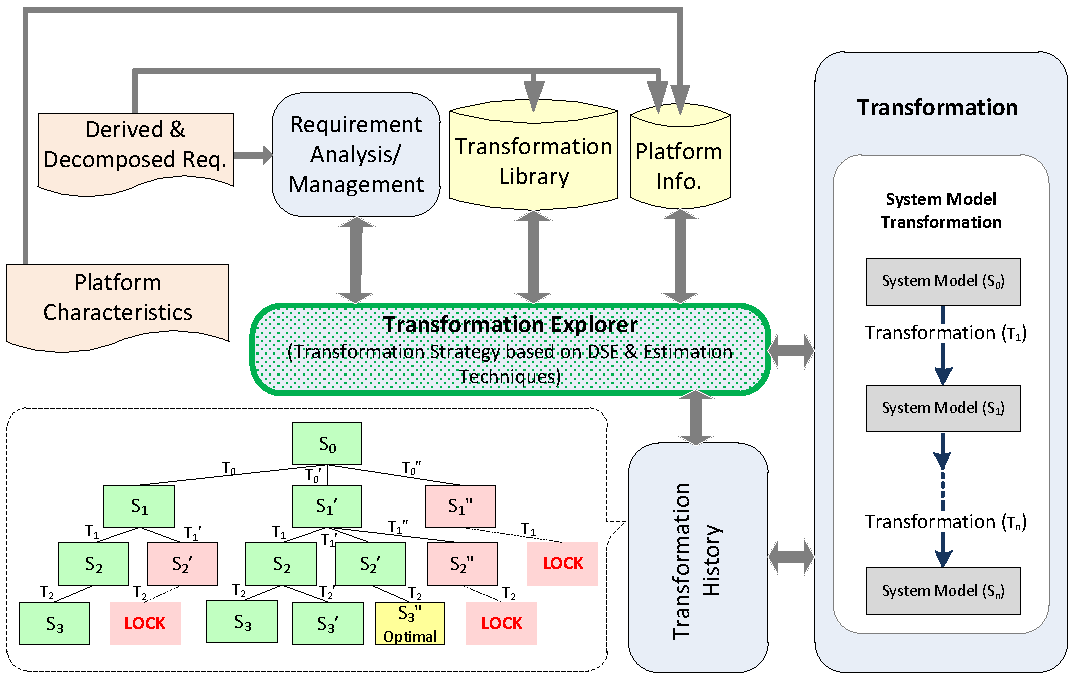
\includegraphics[width=\linewidth]{transformation.pdf}
	\caption{Transformation phase of the proposed methodology.}
	\label{transformation}
\end{figure}

Figure \ref{transformation} illustrates the transformation phase. Apart from derived requirements, another input to the design process are the \textit{Platform Characteristics}, i.e., the reuse of previously used architectures, design rules, guidelines and best practices.
Platform information including processors, memories and interconnection links that are allowed to be used during the platform transformation process are extracted from given platform characteristics. 
This phase mainly focuses on transforming the initial system model (\textit{System Model Transformation}) successively to several intermediate models (\textit{Transformation}).
Transformations are comprised of three steps: 1) pattern recognition: detecting possible transformations, 2) transform: transforming the system model by applying the corresponding transformation rule, and 3) efficient sequence  of  transformations: selecting the most promising sequence  of  transformations by virtue of DSE. The steps are elaborated and exemplified in the following. 

\begin{figure}[t]
%    \captionsetup{position=b}
	\centering
	\includegraphics[width=1.8in]{figs-src/MapMerge.png}
	\caption{The transformation rule ``MapMerge" \cite{sander2003system}.}
	\label{MapMerge}
\end{figure}
\begin{figure*}[t]
	\centering
	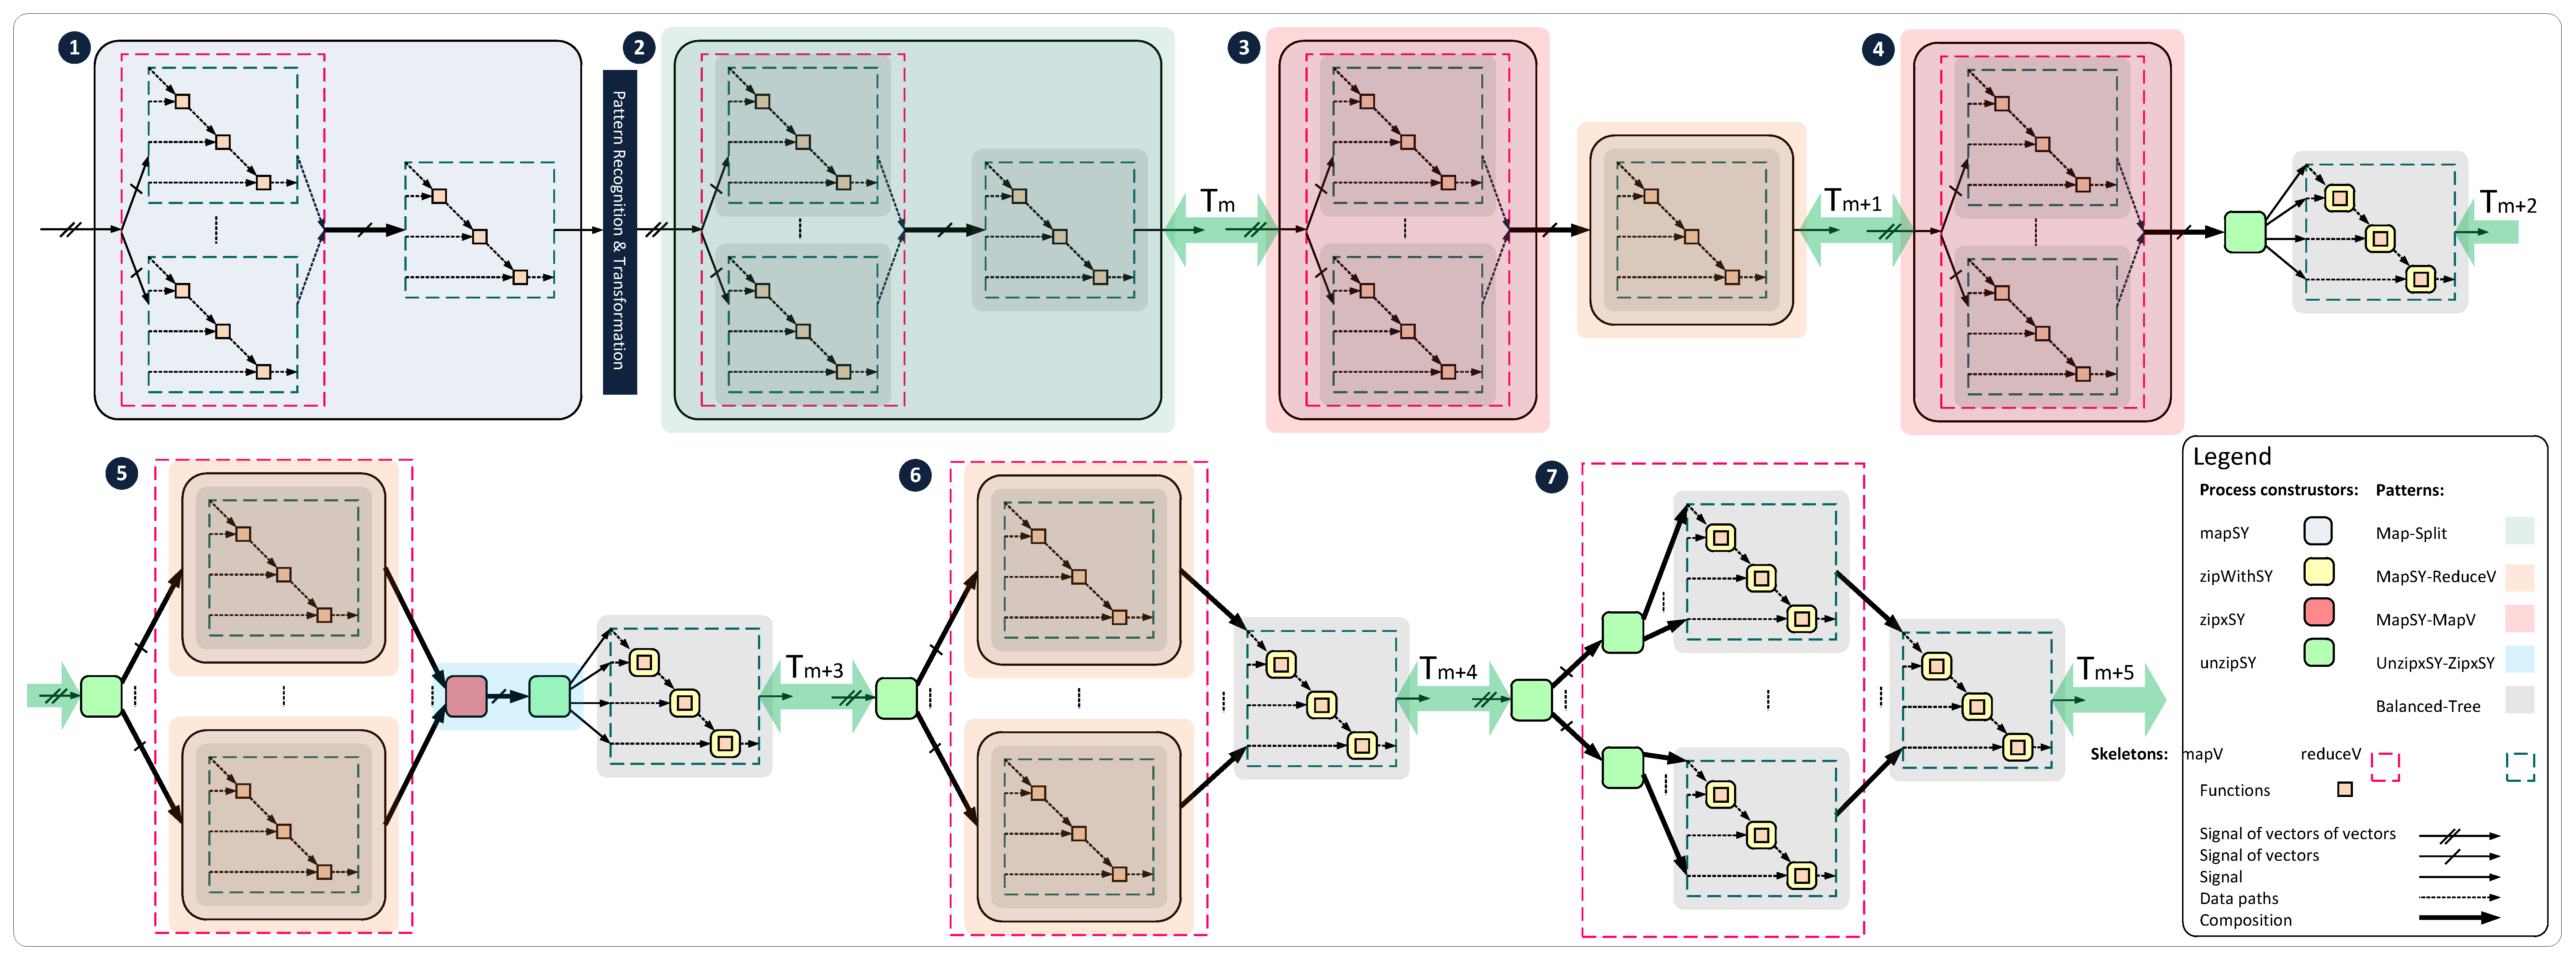
\includegraphics[width=\linewidth]{figs-src/brightness-transformation-flat.pdf}
	\caption{The transformation steps of maxBrightnessSY function.}
	\label{pattern}
\end{figure*}

\subsubsection{Pattern recognition}  
Since the proposed methodology is a rule-based transformational design method, the detection process of possible transformations is done using the patterns predefined in transformation rules. 

\begin{exmp}\label{ex:transformationRule}
As an example of transformation rules of application models, the transformation rule ``MapMerge" from~\cite{sander2003system} is shown in Figure \ref{MapMerge}. This transformation merges two processes. The ``Original Process Networks'' defines the pattern. The ``Transformed Process Network" describes how to transform the original process network.\qed
\end{exmp}

In Figure \ref{transformation}, an envisioned tool \textit{Transformation Explorer} fetches the patterns from \textit{Transformation Library}, explores the application model, and searches for the patterns. 
%It would be well advised to use a graph representation of the models undergoing transformations to be used for pattern recognition and to capture transformation results, as it is easier to transform from/into a graph. 
Defining the platform model-related transformations and enriching the transformation library are beyond the scope of this work and are deferred to future work. 
%In this work we only show how to conduct system developments using our integrated transformation-based methodology.

\begin{exmp}\label{maxBrightness}
Figure \ref{pattern} visualizes the pattern detection and transformation flow in transformation steps $T_m$ to $T_{m+4}$ of the process \texttt{maxBrightnessSY} (Example \ref{ex:appModel}). Patterns are shown by means of transparent colored boxes. The ForSyDe code, implemented in Haskell, of the transformation rules, including the original (patterns) and the transformed processes, used in this paper is given in Listing \ref{transformationRules}. In the following, the rules are  briefly explained.  
\begin{lstlisting}[float,floatplacement=H, language=Haskell, label={transformationRules}, caption= Haskell code of the transformation rules used in this paper.]
-- Transformation rules
-- Original Process = Transformed Process
---------------------------------------------------
-- Transformation Map-Split
mapSY (f . g) = mapSY f . mapSY g
-- Transformation MapSY-ReduceV
mapSY (reduceV f) = reduceV (zipWithSY f) . unzipxSY
-- Transformation MapSY-MapV
mapSY (mapV f) = zipxSY . mapV (mapSY f) . unzipxSY
-- Transformation ZipxSY-UnzipxSY
zipxSY . unzipxSY = id
-- Transformation Balanced-Tree
reduceV f vs = reduceTreeV f vs
reduceTreeV _ (a:>NullV) = a -- single element
reduceTreeV f vs =  -- tree stages recursion
  reduceTreeV f (mapV (reduceV f) (groupV 2 vs))
-- Transformation Serialize-Clock-Domain
delaySY s0 . mapSY (reduceV f)  vs =
downDI (length vs) . mooreSY (f) (id) s0 . par2serxDI
\end{lstlisting}

\begin{itemize}[leftmargin=*]
	\setlength{\parskip}{1pt} 
	\setlength{\itemsep}{0pt plus 0pt}
    \item \texttt{Map-Split}: This rule is the reverse transformation rule of the rule MapMerge (Figure \ref{MapMerge}), and is based on the identity \texttt{mapSY (f . g) = mapSY f . mapSY g} \cite{sander2004system}.
    \item \texttt{MapSY-ReduceV}: Since the ForSyDe compilation rules treat a process as a single entity during synthesis and does not divide a process further, this rule is used to convert a process that includes potential data parallelism, i.e., \texttt{reduceV}, into a parallel process network with the same function.
    \item \texttt{MapSY-MapV}: This rule provides the same benefit as the  rule \texttt{MapSY-ReduceV} does. 
    \item \texttt{ZipxSY-UnzipxSY}: This rule is based on the identity \texttt{zipxSY . unzipxSY = id}, and increases the level of parallelism.
    \item \texttt{Balanced-Tree}: This rule transforms a combinational process to a balanced one. It can be used if the input function is combinational and its operator is associative \cite{sander2004system}.
    \item \texttt{Serialize-Clock-Domain}: This rule \textquote{transforms a combinatorial processes of a regular structure into a structure with two clock domains that uses an FSM process to schedule the operations into several clock cycles} \cite{sander2004system}.
\end{itemize}
Step \circled{1} of Figure \ref{pattern} shows the original process  \texttt{maxBrightnessSY}. Pattern recognition and transformation starts from Step \circled{2}. 
%In the original process network two patterns, related to  transformation rules \texttt{Map-Split} and \texttt{Balanced-Tree} are detected (\circled{2}) and in transformation $T_m$, transformation rule \texttt{Map-Split} is applied, and the transformed process network is illustrated in Step \circled{3}. 
Table \ref{patterndetection} summarizes detected patterns and applied transformations in each step of Figure \ref{pattern}. \qed
\begin{table*}[t]
    \centering
    \caption{Pattern recognition and transformation steps of Figure \ref{pattern}.}
    \begin{tabular}{c||c|c|c}
        \hline
        \textbf{Transformation step} & \textbf{Detected patterns} & \textbf{Selected transformation} & \textbf{Applied transformation} \\
        \hline
        \circled{2} & \texttt{Balanced-Tree}, \texttt{Map-Split} & \texttt{Map-Split} & \circled{2} $\xrightarrow[]{T_m}$ \circled{3}\\
        \hline
        \circled{3} & \texttt{Balanced-Tree}, \texttt{MapSY-MapV}, \texttt{MapSY-ReduceV} & \texttt{MapSY-ReduceV} & \circled{3} $\xrightarrow[]{T_{m+1}}$ \circled{4}\\
        \hline
        \circled{4} & \texttt{Balanced-Tree}, \texttt{MapSY-MapV} & \texttt{MapSY-MapV} & \circled{4} $\xrightarrow[]{T_{m+2}}$ \circled{5}\\
        \hline
        \circled{5} & \texttt{Balanced-Tree}, \texttt{MapSY-ReduceV}, \texttt{ZipxSY-UnzipxSY} & \texttt{ZipxSY-UnzipxSY} & \circled{5} $\xrightarrow[]{T_{m+3}}$ \circled{6}\\
        \hline
        \circled{6} & \texttt{Balanced-Tree}, \texttt{MapSY-ReduceV} & \texttt{MapSY-ReduceV} & \circled{6} $\xrightarrow[]{T_{m+4}}$ \circled{7}\\
        \hline
        \circled{7} & \texttt{Balanced-Tree} & \texttt{Balanced-Tree} & \circled{7} $\xrightarrow[]{T_{m+5}}$ \circled{8}\\
        \hline
    \end{tabular}
    \label{patterndetection}
\end{table*} 
\end{exmp} 
\subsubsection{Transform}
Transformation rules define how to transform the system model. Transformation rules in conjunction with \textit{Transformation History} (Figure \ref{transformation}) provide  transparent transformations, as they enable transformations backward and forward. 
\begin{exmp}
Figure \ref{pattern} shows how the original process \texttt{maxBrightnessSY} is transformed to several intermediate models, using the formats defined as ``transformed process network" in rules. Moreover, Listing \ref{code} shows the transformation of its ForSyDe code. The ForSyDe code of the original image processing application (Figure \ref{appModel}) and that of the transformed application model will be available at GitHub \cite{omitted}.\qed
\begin{lstlisting}[float,floatplacement=H, language=Haskell, label={code}, caption= The transformation of process maxBrightnessSY.]
maxBrightness = mapSY (reduceV f . mapV (reduceV f))
-- Transformation Map-Split
maxBrightness = mapSY (reduceV f) . mapSY (mapV (reduceV f))
-- Transformation MapSY-ReduceV
maxBrightness = reduceV (zipWithSY f) . unzipxSY . mapSY (mapV (reduceV f))
-- Transformation MapSY-mapV
maxBrightness = reduceV (zipWithSY f) . unzipxSY . zipxSY . mapV (mapSY (reduceV f)) . unzipxSY
-- Transformation ZipxSY-UnzipxSY
maxBrightness = reduceV (zipWithSY f) . mapV (mapSY (reduceV f)) . unzipxSY
-- Transformation MapSY-ReduceV
maxBrightness = reduceV (zipWithSY f) . mapV (reduceV (zipWithSY f) . unzipxSY) . unzipxSY
\end{lstlisting}
\end{exmp}
\begin{table*}[t]
    \centering
    \caption{Part of the transformation tree of process maxBrightnessSY.}
    \begin{tabular}{c|c|c}
        \hline
        \multicolumn{3}{c}{\makecell{\textbf{Original system model:} $S_n = (R_i, A_j, M_k, P_l)$, $A_j:reduceV (mapSY f)$, $R_i:t_{prop}\leq60$}}\\
        \hline
        \textbf{Sequence 1} & \textbf{Sequence 2} & \textbf{Sequence 3}\\
        \hline
        \hline
        -&-&\makecell{$S_n = (R_i, A_j, M_k, P_l)$\\$A_j \xrightarrow[]{MapSY-ReduceV} A_{j+1}$}\\
        \hline
        \makecell{$S_n = (R_i, A_j, M_k, P_l)$\\$A_j \xrightarrow[]{Balanced-Tree} A_{j+1}$}&-&\makecell{$S_n = (R_i, A_{j+1}, M_k, P_l)$\\$A_{j+1} \xrightarrow[]{Serialize-Clock-Domain} A_{j+2}$} \\
        \hline
        \makecell{$S_n = (R_i, A_{j+1}, M_k, P_l)$\\$P_l \xrightarrow[]{HW} P_{l+1}$}& \makecell{$S_n = (R_i, A_{j}, M_k, P_l)$\\$P_l \xrightarrow[]{HW} P_{l+1}$}&
        \makecell{$S_n = (R_i, A_{j+2}, M_k, P_l)$\\$P_l \xrightarrow[]{SW} P_{l+1}$}\\
        \hline
        \makecell{$S_n = (R_i, A_{j+1}, M_k, P_{l+1})$\\$M_k \xrightarrow[]{A_{j+1},P_{l+1}} M_{k+1}$} & \makecell{$S_n = (R_i, A_{j}, M_k, P_{l+1})$\\$M_k \xrightarrow[]{A_{j},P_{l+1}} M_{k+1}$} &
        \makecell{$S_n = (R_i, A_{j+2}, M_k, P_{l+1})$\\$M_k \xrightarrow[]{A_{j+2},P_{l+1}} M_{k+1}$}\\
        \hline
        \makecell{$S_n = (R_i, A_{j+1}, M_{k+1}, P_{l+1})$\\$R_i \xrightarrow[]{decompose} R_{i+1}:2*t_t\leq60$} & \makecell{$S_n = (R_i, A_{j}, M_{k+1}, P_{l+1})$\\$R_i \xrightarrow[]{decompose} R_{i+1}:3*t_t\leq60$}&
        \makecell{$S_n = (R_i, A_{j+2}, M_{k+1}, P_{l+1})$\\$R_i \xrightarrow[]{decompose} R_{i+1}:t_{C-Code}\leq 60$}\\
        \hline
        \makecell{$S_n = (R_{i+1}, A_{j+1}, M_{k+1}, P_{l+1})$}& \makecell{$S_n = (R_{i+1}, A_{j}, M_{k+1}, P_{l+1})$}&
        \makecell{$S_n = (R_{i+1}, A_{j+2}, M_{k+1}, P_{l+1})$}\\
        \hline
    \end{tabular}
    \label{sequenceTran}
\end{table*} 
\begin{figure*}[t]
	\centering
	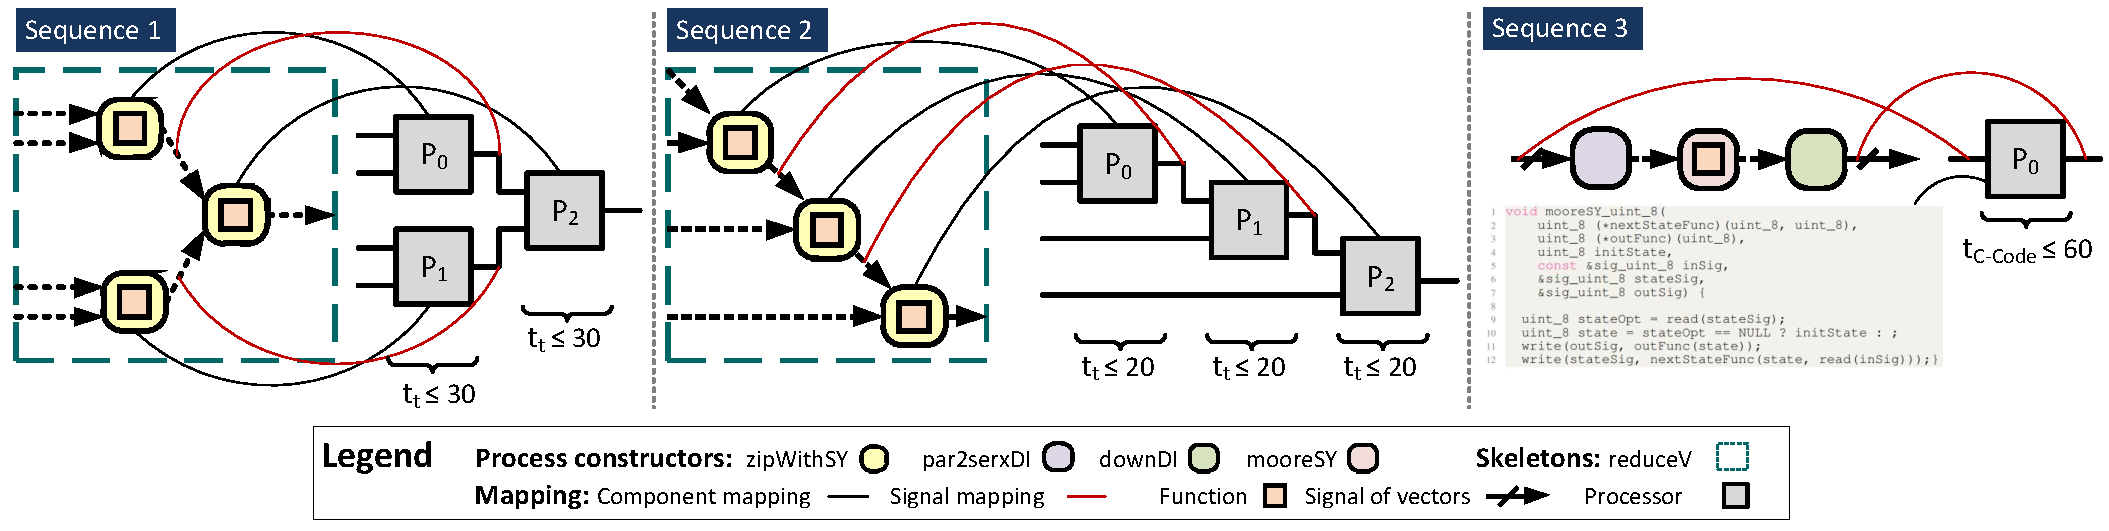
\includegraphics[width=0.986\linewidth]{figs-src/diffSequences.pdf}
	\caption{System models resulted from different sequences of transformations shown in Table \ref{sequenceTran}.}
	\label{sequenceResults}
\end{figure*}
%Exploration: We explore numerous design alternatives to find one that best satisfies ourconstraints. To do this, we  transform the initial de- scription into one moresuitable for implementation. We allocate a set of  system components and specify their  physical and performance constraints, as in  the example in Figure 2, where we allocated three memories, two ASICs, one proces- sor, and several buses. We partition the functional specification among allocated components. For guidance in these exploration subproblems, we estimate each alternative design’s quality \cite{gajski1995specification}.
%In this phase there is no WCETs for the tasks. WCETs come in the mapping model in Phase B.%PIM: list of functions

\subsubsection{Efficient sequence  of  transformations}
In Table \ref{patterndetection}, in Steps~\circled{2} to \circled{6}, there is always more than one possible transformation. The applied sequence of  transformations highly affects the implementation. Transforming different parts of the system model provides the opportunity to explore a large number of design alternatives and to achieve an efficient implementation. As a guideline in exploring these sub-problems, we take advantage of early stage DSE, at the higher abstraction levels where there is no detailed knowledge about the implementation platform, and traditional DSE techniques \cite{pimentel2016exploring}, at the lower levels.
\begin{exmp}
Table \ref{sequenceTran} shows part of the transformation tree of process \texttt{maxBrightnessSY}, i.e., \texttt{reduceV~(mapSY f)}, as three different sequences of transformations, and Figure~\ref{sequenceResults} illustrates the system model resulting from each of them.
For each sequence of transformations, Table~\ref{sequenceTran} shows how the original system model, represented in the RAMP-format, is transformed by a step-wise application of transformation rules. 
In sequence 1, the transformation rule \texttt{Balanced-Tree} is used and a hardware implementation is preferred. However, in sequence 2,  a hardware implementation of the original application model is selected. Finally, in sequence 3, after transformation \texttt{Serialize-Clock-Domain} (Listing \ref{transformationRules}), the application model includes the process \texttt{mooresy (max) (id) 0} constructed by process constructor \texttt{mooreSY}, which is interpreted as a FSM \cite{sander2004system}. The software implementation (C-code) of the application model is mapped to a single core. Figure \ref{sequenceResults} also shows the transformations of requirements, where the top-level requirement $R_i:t_{prop}\leq60$ has been transformed into derived requirements on the individual sub-systems. 

In this step, DSE techniques are used to estimate the quality of each implementation and define the most promising one. \qed
%For the platform model, annotated components from the component library are used. 
\end{exmp}




%\begin{itemize}
%    \item Initial platform:
%    \begin{itemize}
%        \item @SAAB: Initial platform is needed (memory, bandwidth, ...).
%        \item @Ingo: Initial platform is an empty platform.
%        \item @Fahimeh: one single node.
%    \end{itemize}
%    \item The initial contract $C_0$: formal specification of requirements.
%\end{itemize}


%Phase B mainly focus on transforming the initial models of the application, platform, mapping, and refined requirements (\textit{System Model transformation})  successively to several intermediate models (\textit{Transformation}). Transformations are comprised of three steps: 1) detecting possible transformations, 2) selecting one of them to be applied in the next transformation step, 3) refining the system model. 
%We propose a transformation strategy for the first and second task and a rule-based transformation approach for the third one as follows:

%\begin{itemize}
% \item \textbf{Transformation strategy:}
% The detection process of possible transformations is done by means of the paterns pre-identified by the transformation rules. Moreover, the refinemnts of both the application model and the platform model follow the composition rules defined by the underlying modeling framework. In other owrds, the initial application model fed into Phase B is a process network, i.e., a functional composition of processes. 
% For  such application models that are based on the features defined in Section \ref{sec:application model}, process constructors identify applicable composition patterns. Also, platform models, supporting compositional transformation, follow the composition rules stored in the \textit{Platform Information} library, as well as defining some notations of dominance to help for detecting pareto-compositinal transformations of the components. It would be well advised to use a graph representation of the models undergoing transformations to capture transformation results as it is easier to transform from/into a graph. To detect the possible transformations, Transformation Explorer explores the graph representation of the system model and search for the patterns. 

 
%The transformation tree shown in Phase B of Figure \ref{Sequence} illustrates the complexity of the first two steps of each transformation. It is the transformation tree of a transformation library including only three transformation rules, i.e., $\{T, T', T''\}$. In the first transformation step, transformations $T_0$ and $T'_0$ are possible. It is possible to either try both of them out or to select the transformation that is dominant in the current transformation step.  The first strategy is a comprehensive solution that leads to an optimal solution, while the second one ensures at least a \textit{good enough} solution that can be the optimal solution, as well. The proposed transformation strategy follows the second strategy and select one of the possible transformations by virtue of a \textit{Transformation Explorer} to transform the system model in a timely manner. The transformation explorer first filters the transformations that do not satisfy requirements out and then takes advantage of \textit{Refined Requirements}, \textit{Early-stage DSE}, and \textit{Estimation Techniques} to find the pareto-refinemnt. 


  
 %\item \textbf{transformation:}
% TRANSFORM is a rule-based transformation methodology. The rules define the formats of the original  (patterns) and refined process networks as well as the implication of the design transformation. The implications pave the way for verifying the transformations. It is also worth mentioning that the transformation rules filling the transformation library are highly dependent on the application domain. A clear understanding of the underlying application domain is extremely important and necessary to design suitable transformation rules.  
%\end{itemize}

 
 

%For example, given an in-termediate result represented in ETPN, an algorithm can be used to estimate its implementation cost, checkwhether that satisfies the design constraints, and automatically choose a transformation to apply to the de-sign which produces another intermediate result with improved cost. ETPN, for example, is used by theCAMAD hardware synthesis system [Pen 88b] to support an iterative transformation approach to carry outthe synthesis tasks. CAMAD first generates a preliminary (default) design in ETPN format from the inputspecification. It then applies transformations one by one to the preliminary result so as to obtain better so-lutions. This iterative process is finished when satisfactory results have been reached. The data path is thentransformed  into  a  net-list  and  the  control  Petri  net  into  a  microprogram.  The  proposed  silicon/softwarecompiler environment will use the same strategy \cite{peng1991unified}.
%Synthesis can further besplit into 1) decision making, which is theeducated(i.e. anaylsis-based) process ofsteering the design flow; and 2) transformation, which is the task of incorporating thesedecision into the behavioral model, resulting into an implementation model.


%very important: learning
%Product design decisions based on performance needs
%Dependencies between requirements must be tracked.
%Keeping history of transformations: The  design  process  and  design  decisions  are documented,   thus   the   whole   process   is repeatable \cite{wu2001transformational}.
%In particular, a design methodology should separate:1) function (what the system is supposed to do) from architecture (how it does it) and 2) communication from computation \cite{sander2004system}.
%based on the platform characteristics and platform info., the expected worst case execution time of each task on each processing element can be calculated. 
%when there are dual-criticality tasks, at least three nodes are needed.
%transform heavily relays on design rules. Design rules also speed up DSE.
%\subsection{Phase C}

% $mapV (mapSY f)$ should be mapped on GPU (since it is a stream processing 

%Accelerator: For      example,      in      HW/SW      co-design,transformation  techniques  can  be  employed  inthe system's custom parts that are not covered bypre-designed building blocks (IPs).

%The last paragraph: Of course, there are still difficulties in applying apurely transformational approach to large systemdesign.   However,   the   incorporation   of   thisapproach  into  the  design  methodology  will  offerthe  opportunities  to  improve  the  design  process \cite{wu2001transformational}.

%should the figure be changed to include mapping and design constraint transformations as well?


%\begin{lstlisting}[float,floatplacement=H, language=C++, label={code}, caption= The transformation of process maxBrightnessSY.]
%void mooreSY_uint_8(
%    uint_8 (*nextStateFunc)(uint_8, uint_8),
%    uint_8 (*outFunc)(uint_8),
%    uint_8 initState,
%    const &sig_uint_8 inSig,
%    &sig_uint_8 stateSig,
%    &sig_uint_8 outSig) {

%  uint_8 stateOpt = read(stateSig);
%  uint_8 state = stateOpt == NULL ? initState : ;
%  write(outSig, outFunc(state));
%  write(stateSig, nextStateFunc(state, read(inSig)));}
%\end{lstlisting}


%%% Local Variables:
%%% mode: latex
%%% TeX-master: "../paper"
%%% End:

\section{Conclusion}
\label{sec:conclusion}
The paper has extended existing transformational design approaches into a novel system design methodology. A key idea is to center the methodology around a coherent system model view (\textit{RAMP}), where the system at each transformation step is expressed as a tuple of requirements, application model, platform model, and mapping model. This enables to systematically refine both application and platform model, which significantly increases the potential to identify an efficient implementation. The main concepts and mechanisms of the method have been illustrated by a representative example. Future work will cover the development of tool support for the methodology and an extension of the transformation library.
%Future work: safety aspects.
%We have extended and wrapped exiting transformation-based approaches in a systematic fully transformational design methodology. The proposed methodology transforms different parts of the system model, \textit{RAMP}, and traverses numerous design points. A pattern recognition method is used as a lever to detect potential transformations, which in turn show the design alternatives up. A running example of an image processing application has demonstrated how to apply step-wise transformations to develop a system. Although the example shows the potentials of the methodology, it is definitely needed to design application-specific transformation rules. Future work will focus on automation of the methodology and  enriching the transformation library. Pattern recognition tool is under development. 
%It is also true that a formal  
%%% Local Variables:
%%% mode: latex
%%% TeX-master: "../paper"
%%% End:


%\section*{Acknowledgment}

%The preferred spelling of the word ``acknowledgment'' in America is without an ``e'' after the ``g''. Avoid the stilted expression ``one of us (R. B. G.) thanks $\ldots$''. Instead, try ``R. B. G. thanks$\ldots$''. Put sponsor acknowledgments in the unnumbered footnote on the first page.

\bibliographystyle{IEEEtran}\bibliography{references/ref}

\end{document}


%%% Local Variables:
%%% mode: latex
%%% TeX-master: t
%%% End:
